\باب{اینٹینا اور شعاعی اخراج}

\حصہ{تعارف}

\حصہ{تاخیری دباو}
کسی بھی اخراج شعاع کے نظام میں موج کے ترسیل کے لئے درکار دورانیہ اہمیت رکھتا ہے۔یوں شکل \حوالہ{شکل_اینٹینا_تاخیری_رو} میں دکھائے تار میں برقی رو سے پیدا میدان کا اثر نقطہ \عددیء{N} پر کچھ وقفے سے ہو گا۔خالی خلاء میں یہ وقفہ موج کو تار سے نقطے تک پہنچنے کا دورانیہ \عددیء{\frac{r}{c}} ہے جہاں
 \عددیء{c=\SI{3e8}{\meter/\second}} خالی خلاء میں  شعاع کی رفتار ہے۔یوں \عددیء{N} کے نقطہ نظر سے تار میں برقی رو
\begin{align}
I=I_0 \cos \omega t
\end{align} 
کی بجائے
\begin{align}\label{مساوات_اینٹینا_تاخیری_رو}
[I]=I_0 \cos \omega  \left (t-\frac{r}{c} \right)
\end{align} 
لکھی جا سکتی ہے جہاں \عددیء{[I]} \اصطلاح{تاخیری برقی رو}\فرہنگ{تاخیری!برقی رو}\حاشیہب{retarded current}\فرہنگ{retarded!current} کہلاتی ہے۔تاخیری تفاعل کو چکور قوسین میں بند لکھا جاتا ہے۔تاخیری برقی رو لکھتے ہوئے وقت \عددیء{t} کی جگہ تاخیری وقت \عددیء{(t-\tfrac{r}{c})} استعمال کیا جاتا ہے۔

\begin{figure}
\centering
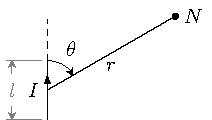
\includegraphics{figAntennaRetardedCurrent}
\caption{برقی رو گزارتی تار کی چھوٹی لمبائی}
\label{شکل_اینٹینا_تاخیری_رو}
\end{figure}

مساوات \حوالہ{مساوات_اینٹینا_تاخیری_رو} کہتا ہے کہ نقطہ \عددیء{N} پر لمحہ \عددیء{t}  پر پیدا اثر،  گزرے  لمحے \عددیء{(t-\tfrac{r}{c})} پر تار میں برقی رو کا اثر ہے جہاں تار سے \عددیء{N} تک فاصلہ \عددیء{r} ہے۔تار سے \عددیء{N} تک شعاع پہنچنے کا دورانیہ \عددیء{\tfrac{r}{c}} ہے۔

گزشتہ بابوں میں امواج کی بات کرتے ہوئے \عددیء{\cos (\omega t -\beta x)} استعمال کیا گیا جس میں \عددیء{\tfrac{\omega}{\beta}=c} کے استعمال سے
\begin{align}
\cos (\omega t -\beta x)=\cos \omega\left( t- \frac{x}{c}\right)
\end{align}
لکھا جا سکتا ہے  جو تاخیری تفاعل کو ظاہر کرتی ہے۔

مساوات \حوالہ{مساوات_اینٹینا_تاخیری_رو} کی دوری سمتیہ شکل
\begin{align}
[I]=I_0 e^{j \omega (t-r/c)}=I_0 e^{j(\omega t-\beta r)}
\end{align}
ہے۔اسی طرح کثافت برقی رو کی تاخیری دوری سمتیہ شکل
\begin{align}
[\kvec{J}]=\kvec{J}_0 e^{j \omega (t-r/c)}=\kvec{J}_0 e^{j(\omega  t -\beta r)}
\end{align}
ہو گی جسے استعمال کرتے ہوئے تاخیری مقناطیسی دباو
\begin{align}\label{مساوات_اینٹینا_تاخیری_سمتی_دباو}
[\kvec{A}]=\frac{\mu}{4\pi}\int_h \frac{[\kvec{J}]}{r}\dif h=\frac{\mu}{4\pi}\int_h \frac{\kvec{J}_0 e^{j\omega(t-r/c)}}{r} \dif h
\end{align}
لکھا جائے گا۔اسی طرح تاخیری حجمی کثافت چارج
\begin{align}
[\rho_h]= \rho_0 e^{j\omega \left(t-r/c \right)}
\end{align}
لکھتے ہوئے تاخیری برقی دباو
\begin{align}\label{مساوات_اینٹینا_تاخیری_مقداری_دباو}
[V]=\frac{1}{4\pi \epsilon}\int_h \frac{[\rho_h]}{ r} \dif h
\end{align}
لکھا جائے گا۔ باب-\حوالہ{باب_میکس_ویل} کے آخر میں مساوات \حوالہ{مساوات_میکس_ویل_تاخیری_سمتی_دباو} اور مساوات \حوالہ{مساوات_میکس_ویل_تاخیری_غیر_سمتی_دباو} کے بائیں ہاتھ کے تفاعل کو چکور قوسین میں لکھ کر موج کی رفتار \عددیء{c} لیتے ہوئے اور فاصلے  کو کروی محدد کے رداس \عددیء{r} سے ظاہر کرنے سے  یہی مساوات حاصل ہوتے ہیں۔


\حصہ{مختصر جفت قطبی اینٹینا}
مختصر لمبائی کے سیدھے موصل تار کو عموماً مختصر \اصطلاح{ جفت قطب}\فرہنگ{جفت قطب!مختصر}\حاشیہب{short dipole}\فرہنگ{dipole!short} کہا جاتا ہے۔مندرجہ ذیل گفتگو میں مختصر جفت قطب کی لمبائی محدود ہو گی۔لامحدود حد تک کم لمبائی کی صورت میں اسے صغاری جفت قطب\فرہنگ{صغاری جفت قطب}\حاشیہب{infinitesimal} کہا جائے گا۔

خطی نوعیت کے کسی بھی اینٹینا کو متعدد تعداد کے سلسلہ وار جڑے مختصر جفت قطبوں کا مجموعہ تصور کیا جا سکتا ہے لہٰذا مختصر جفت قطب کی خاصیت جانتے ہوئے زیادہ لمبے جفت قطب یا مختلف انداز میں جڑے موصل  تاروں کی خاصیت جاننے میں مدد ملے گی۔ 

آئیں شکل \حوالہ{شکل_اینٹینا_جفت_قطب}-الف میں دکھائے مختصر جفت قطب پر غور کریں جس کی لمبائی \عددیء{l} طول موج سے بہت کم \عددیء{l\ll \lambda} ہے۔جفت قطب کے سروں پر موصل چادر بطور  کپیسٹر  بوجھ کردار ادا کرتے ہیں۔جفت قطب کی مختصر لمبائی اور اس کے سروں پر موصل چادر مل کر جفت قطب  کی پوری لمبائی پر تقریباً برابر برقی رو رکھنے میں مدد دیتے ہیں۔جیسے شکل-الف میں دکھایا گیا ہے، جفت قطب کو متوازن ترسیلی تار سے طاقت مہیا کی جا سکتی ہے۔یہ فرض کرتے ہوئے کہ ترسیلی تار سے شعاعی اخراج نہیں ہوتی، اس کے موجودگی کو نظر انداز کیا جائے گا۔جفت قطب کے سروں پر نسب موصل چادروں کے شعاعی اخراج کو بھی نظر انداز کیا جائے گا۔جفت قطب کی موٹائی \عددیء{d} اس کے لمبائی سے بہت کم \عددیء{d\ll \lambda} ہے۔ان حقائق کو مد نظر رکھتے ہوئے تحلیلی تجزیے کی خاطر جفت قطب کو شکل \حوالہ{شکل_اینٹینا_جفت_قطب}-ب کی طرح تصور کیا جا سکتا ہے۔ایسا جفت قطب یکساں برقی رو \عددیء{I} گزارتا، \عددیء{l} لمبائی کا تار معلوم ہو گا جس کے دونوں سروں پر برابر مگر الٹ قطب کے چارج \عددیء{\mp q} ہوں۔کپیسٹر پر چارج \عددیء{q} اور برقی رو \عددیء{I} کا تعلق
\begin{align}\label{مساوات_اینٹینا_رو_اور_چارج}
I=\frac{\partial q}{\partial t}
\end{align}
ہے۔ 

آئیں لامحدود وسعت کی خالی خلاء میں جفت قطب کے میدان حاصل کریں۔جفت قطب کے وسط کو کروی محدد کے مرکز اور لمبائی کو \عددیء{z} محدد پر رکھتے ہوئے آگے بڑھتے ہیں۔کسی بھی نقطہ \عددیء{N} پر عموماً آپس میں عمودی تین میدان \عددیء{E_r}، \عددیء{E_{\theta}} اور \عددیء{E{\phi}} پائے جائیں گے۔

\begin{figure}
\centering
\begin{subfigure}{0.4\textwidth}
\centering
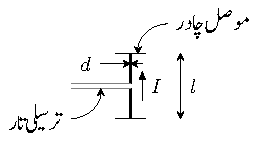
\includegraphics{figAntennaShortDipole}
\caption*{الف: متوازن ترسیلی تار سے جفت قطب کو طاقت مہیا کی گئی ہے۔}
\end{subfigure}%
%
\begin{subfigure}{0.4\textwidth}
\centering
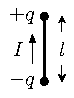
\includegraphics{figAntennaShortDipoleAsShortWire}
\caption*{ب: جفت قطب بطور چھوٹی تار}
\end{subfigure}%
\caption{جفت قطب}
\label{شکل_اینٹینا_جفت_قطب}
\end{figure}


کسی بھی نقطہ \عددیء{N} پر مساوات \حوالہ{مساوات_میکس_ویل_تاخیری_مقناطیسی_میدان}  اور مساوات \حوالہ{مساوات_میکس_ویل_تاخیری_برقی_میدان} بالترتیب مقناطیسی میدان اور برقی میدان دیتے ہیں
\begin{align}
\kvec{H}=\frac{1}{\mu_0}\nabla \times \kvec{A} \\
\kvec{E}=-\nabla V-\frac{\partial \kvec{A}}{\partial t}
\end{align}
جہاں
\begin{description}
\جزو{$V$} نقطہ \عددیء{N} پر مقداری برقی دباو
\جزو{$\kvec{A}$} نقطہ \عددیء{N} پر سمتی دباو
\end{description}
ہیں۔اگر ہمیں کسی بھی نقطے پر مقداری دباو \عددیء{V} اور سمتی دباو \عددیء{\kvec{A}} معلوم ہوں تب مندرجہ بالا دو مساوات سے اس نقطے پر برقی اور مقناطیسی میدان حاصل کئے جا سکتے ہیں۔چونکہ ہمیں  جفت قطب سے دور میدان درکار ہیں لہٰذا ایسی صورت میں مساوات \حوالہ{مساوات_اینٹینا_تاخیری_سمتی_دباو} اور مساوات \حوالہ{مساوات_اینٹینا_تاخیری_مقداری_دباو} میں دئے تاخیری دباو قابل استعمال ہوں گے۔یوں ان مساوات کو
\begin{align}
\kvec{H}&=\frac{1}{\mu_0}\nabla \times [\kvec{A}] \label{مساوات_اینٹینا_عمومی_مقناطیسی}\\
\kvec{E}&=-\nabla [V]-\frac{\partial [\kvec{A}]}{\partial t}=-\nabla [V]-j \omega [\kvec{A}]\label{مساوات_اینٹینا_عمومی_برقی}
\end{align}
لکھا جا سکتا ہے جہاں مساوات \حوالہ{مساوات_میکس_ویل_بدلتا_میدان_غیر_سمتی_دباو} اور مساوات \حوالہ{مساوات_میکس_ویل_بدلتا_میدان_سمتی_دباو} سے تاخیری دباو
\begin{align}
[\kvec{A}]&=\frac{\mu_0}{4\pi} \int_h \frac{\kvec{J}_0 e^{j \omega(t-r/c)}}{r} \dif h \label{مساوات_اینٹینا_عمومی_سمتی_دباو}\\
[V]&=\frac{1}{4\pi\epsilon_0}\int_h \frac{\rho_0 e^{j\omega(t-r/c)}}{r} \dif h\label{مساوات_اینٹینا_عمومی_مقداری_دباو}
\end{align}
لکھے جا سکتے ہیں۔

کسی بھی برقی چارج اور برقی رو سے پیدا میدان مساوات \حوالہ{مساوات_اینٹینا_عمومی_مقناطیسی} اور مساوات \حوالہ{مساوات_اینٹینا_عمومی_برقی} سے حاصل کئے جا سکتے ہیں۔مساوات \حوالہ{مساوات_اینٹینا_عمومی_مقداری_دباو} کے تحت تاخیری مقداری دباو \عددیء{[V]} صرف ساکن چارجوں پر منحصر ہے جبکہ مساوات \حوالہ{مساوات_اینٹینا_عمومی_سمتی_دباو} کے تحت  تاخیری سمتی دباو \عددیء{[\kvec{A}]} صرف برقی رو یعنی حرکت کرتے چارجوں پر منحصر ہے۔مساوات \حوالہ{مساوات_اینٹینا_عمومی_مقناطیسی} کے تحت مقناطیسی میدان \عددیء{\kvec{H}} صرف برقی رو یعنی حرکت کرتے چارجوں پر منحصر ہے جبکہ مساوات \حوالہ{مساوات_اینٹینا_عمومی_برقی} کے تحت برقی میدان \عددیء{\kvec{E}} ساکن چارج اور برقی رو دونوں پر منحصر ہے۔ہم جلد دیکھیں گے کہ کسی بھی چارج اور برقی رو سے  دور پیدا مقناطیسی اور برقی میدانوں کا دارومدار صرف برقی رو پر ہوتا ہے۔ چونکہ اس باب میں تاخیری دباو ہی استعمال کئے جائیں گے لہٰذا انہیں چکور قوسین میں لکھنے سے گریز کیا جائے گا۔اس باب میں یہاں سے آگے بغیر چکور قوسین کے دباو کو تاخیری دباو ہی سمجھا جائے۔

شکل سے ظاہر ہے کہ سمتی دباو کا صرف \عددیء{\az} جزو
\begin{align}
\kvec{A}=\frac{\az \mu_0 I_0}{4\pi} \int_{-l/2}^{l/2} \frac{e^{j(\omega t -\beta s)}}{s} \dif z
\end{align}
 پایا جاتا ہے۔اگر جفت قطب کی لمبائی \عددیء{l}، نقطہ \عددیء{N} سے جفت قطب تک فاصلہ \عددیء{r} سے نہایت کم \عددیء{l\ll r} اور طول موج \عددیء{\lambda} سے بھی نہایت کم \عددیء{l \ll \lambda} ہو تب مندرجہ بالا مساوات میں متغیر فاصلہ \عددیء{s} کی جگہ مستقل فاصلہ \عددیء{r} پر کیا جا سکتا ہے اور ساتھ ہی ساتھ \عددیء{l} پر مختلف نقطوں سے  \عددیء{N} پر پیدا دباو میں زاویائی فرق کو نظر انداز کیا جا سکتا ہے۔یوں مندرجہ بالا مساوات سے
\begin{align}
\kvec{A} =\frac{\az \mu_0 I_0 l e^{j(\omega t -\beta r)}}{4\pi r}
\end{align}
حاصل ہوتا ہے۔ اس مساوات کو کروی محدد میں یوں
\begin{align*}
\kvec{A}=A_r \ar +A_{\theta} \atheta +A_{\phi} \aphi
\end{align*}
لکھا جائے گا جہاں
\begin{gather}
\begin{aligned}\label{مساوات_اینٹینا_کروی_سمتی_دباو}
A_r&=\ar \cdot \kvec{A}= \frac{ \mu_0 I_0 l e^{j(\omega t -\beta r)}}{4\pi r} \ar \cdot \az= \frac{ \mu_0 I_0 l e^{j(\omega t -\beta r)}}{4\pi r} \cos \theta\\
A_{\theta}&=\atheta \cdot \kvec{A}=\frac{ \mu_0 I_0 l e^{j(\omega t -\beta r)}}{4\pi r} \atheta \cdot \az =-\frac{ \mu_0 I_0 l e^{j(\omega t -\beta r)}}{4\pi r} \sin \theta \\
A_{\phi}&=\aphi \cdot \kvec{A}=\frac{ \mu_0 I_0 l e^{j(\omega t -\beta r)}}{4\pi r} \aphi \cdot \az =0
\end{aligned}
\end{gather}
ہوں گے جہاں اکائی سمتیات کے مقداری ضرب صفحہ \حوالہصفحہ{جدول_سمتیہ_کروی_نلکی_اکائی_غیر-سمتی_ضرب} پر جدول \حوالہ{جدول_سمتیہ_کروی_نلکی_اکائی_غیر-سمتی_ضرب} سے حاصل کئے گئے۔اس طرح 
\begin{align}\label{مساوات_اینٹینا_جفت_قطب_سمتی_دباو}
\kvec{A}=\frac{ \mu_0 I_0 l e^{j(\omega t -\beta r)}}{4\pi r}\left(\cos \theta \ar-\sin \theta \atheta \right)
\end{align}
لکھا جائے گا۔

ساکن چارج جفت قطب کے سروں پر پایا جاتا ہے لہٰذا مقداری دباو
\begin{align}\label{مساوات_اینٹینا_مقداری_دباو_الف}
V=\frac{q_0}{4\pi \epsilon_0} \left[\frac{e^{j(\omega t -\beta s_1)}}{s_1} -\frac{e^{j(\omega t -\beta s_2)}}{s_2}\right]
\end{align}
ہو گا جہاں مساوات \حوالہ{مساوات_اینٹینا_رو_اور_چارج} کے تحت
\begin{align}\label{مساوات_اینٹینا_رو_اور_چارج_ب}
q=\int I \dif t=\frac{I}{j\omega }
\end{align}
کے برابر ہے جہاں
\begin{align*}
I&=I_0 e^{j(\omega t -\beta s)}\\
q&=q_0  e^{j(\omega t -\beta s)}
\end{align*}
ہیں۔مساوات \حوالہ{مساوات_اینٹینا_رو_اور_چارج_ب} سے \عددیء{q_0=\tfrac{I_0}{j\omega}} حاصل کرتے ہوئے مساوات \حوالہ{مساوات_اینٹینا_مقداری_دباو_الف} میں پر کرتے ہیں۔ 
\begin{align}\label{مساوات_اینٹینا_مقداری_دباو_ب}
V=\frac{I_0}{4\pi \epsilon_0 j \omega } \left[\frac{e^{j(\omega t -\beta s_1)}}{s_1} -\frac{e^{j(\omega t -\beta s_2)}}{s_2}\right]
\end{align}
شکل کو دیکھ کر
\begin{align*}
s_1&=r-\frac{l}{2}\cos \theta\\
s_2&=r+\frac{l}{2}\cos \theta
\end{align*}
لکھے جا سکتے ہیں جنہیں مساوات \حوالہ{مساوات_اینٹینا_مقداری_دباو_ب} میں پر کرتے
\begin{align}
V=\frac{I_0 e^{j(\omega t -\beta r)}}{4\pi \epsilon_0 j \omega}\left[\frac{(r+\frac{l}{2}\cos \theta) e^{j\frac{\beta l}{2}\cos \theta}-(r-\frac{l}{2}\cos \theta) e^{-j\frac{\beta l}{2}\cos \theta}}{r^2-\frac{l^2}{4}\cos^2 \theta} \right]
\end{align}
ملتا ہے۔چکور قوسین میں شرح کے نچلے حصے میں \عددیء{r \gg l} کی وجہ سے  \عددیء{\tfrac{l^2}{4}\cos^2 \theta} کو نظر انداز کرتے ہیں۔\اصطلاح{مسئلہ ڈی مویور}\فرہنگ{مسئلہ!ڈی مویور}\فرہنگ{ڈی مویور!مسئلہ}\حاشیہب{$(e^{j\alpha}=\cos \alpha + j \sin \alpha)$ de Moivre's theorem}\فرہنگ{de Moivre} کے استعمال سے
\begin{multline}\label{مساوات_اینٹینا_مقداری_دباو_پ}
V=\frac{I_0 e^{j(\omega t -\beta r)}}{4\pi \epsilon_0 j \omega r^2} \left[\left(r+\frac{l}{2}\cos \theta\right) \left(\cos \frac{\beta l \cos \theta}{2} +j \sin \frac{\beta l \cos \theta}{2}\right)\right.\\
-\left.\left(r-\frac{l}{2}\cos \theta\right) \left(\cos \frac{\beta l \cos \theta}{2} -j \sin \frac{\beta l \cos \theta}{2}\right) \right]
\end{multline}  
لکھا جائے گا۔چونکہ \عددیء{l \ll \lambda} ہے لہٰذا 
\begin{align*}
\cos \frac{\beta l \cos \theta}{2}&=\cos \frac{\pi l \cos \theta}{\lambda}\approx l\\
\sin \frac{\beta l \cos \theta}{2}&\approx \frac{\beta l \cos \theta}{2}
\end{align*}
ہوں گے، جنہیں مساوات \حوالہ{مساوات_اینٹینا_مقداری_دباو_پ} میں پر کرنے سے
\begin{align}\label{مساوات_اینٹینا_مقداری_دباو_ت}
V=\frac{I_0 l e^{j(\omega t -\beta r)} \cos \theta}{4\pi \epsilon_0 c}\left(\frac{1}{r}+\frac{c}{j\omega r^2} \right)
\end{align}
حاصل ہوتا ہے جہاں
\begin{description}
\جزو{$I_0$} برقی رو کا حیطہ یعنی اس کی زیادہ سے زیادہ قیمت، \عددیء{\si{\ampere}}
\جزو{$l$} جفت قطب کی لمبائی، \عددیء{\si{\meter}}
\جزو{$\omega$}  زاویائی تعدد \عددیء{(\omega=2\pi f)} ، اکائی \عددیء{\si{\radian / \second}}۔ جہاں ہرٹز \عددیء{\si{\hertz}}میں تعدد \عددیء{f} ہے
\جزو{$\beta$} زاویائی مستقل \عددیء{(\beta=\tfrac{2\pi}{\lambda})}، اکائی \عددیء{\si{\radian /\meter}}
\جزو{$t$}وقت،\عددیء{\si{\second}} 
\جزو{$\theta$}جفت قطب اور جفت قطب سے نقطہ \عددیء{N} تک سمتیہ کے مابین زاویہ
\جزو{$\epsilon_0$}خالی خلاء کا برقی مستقل، \عددیء{\SI{8.854}{\pico\farad/\meter}}
\جزو{$c$}خالی خلاء میں شعاع کی رفتار، \عددیء{\SI{3e8}{\meter/\second}}
\جزو{$j$}خیالی عدد \عددیء{\sqrt{-1}}
\جزو{$r$}جفت قطب کے وسط سے نقطہ \عددیء{N} تک فاصلہ،\عددیء{\si{\meter}}
\end{description}
ہیں۔

مختصر جفت قطب کے وسط سے، \عددیء{l \ll \lambda} اور \عددیء{l \ll r} کی صورت میں، \عددیء{r} فاصلے اور \عددیء{\theta} زاویے پر مساوات \حوالہ{مساوات_اینٹینا_جفت_قطب_سمتی_دباو} سمتی دباو اور مساوات \حوالہ{مساوات_اینٹینا_مقداری_دباو_ت} مقداری دباو دیتے ہیں۔کروی محدد میں مقداری دباو کی ڈھلوان
\begin{gather}
\begin{aligned}
\nabla V&=\frac{\partial V}{\partial r}\ar+\frac{1}{r}\frac{\partial V}{\partial \theta}\atheta+\frac{1}{r\sin \theta} \frac{\partial V}{\partial \phi}\aphi\\
&=\frac{I_0 l e^{j(\omega t -\beta r)}}{4\pi \epsilon_0 c}\left[-\left(\frac{ \cos \theta}{r^2}+\frac{2 c  \cos \theta}{j\omega r^3} \right)\ar -\left(\frac{\sin \theta}{r}+\frac{c \sin \theta}{j\omega r^2} \right) \atheta\right]
\end{aligned}
\end{gather}
کے برابر ہے۔برقی میدان \عددیء{\kvec{E}=E_r \ar +E_{\theta} \atheta+E_{\phi}\aphi} کے اجزاء مساوات \حوالہ{مساوات_اینٹینا_عمومی_برقی} کی مدد سے 
\begin{align*}
E_r&=-\frac{\partial V}{\partial r}-j \omega A_r\\
E_{\theta}&=-\frac{1}{r}\frac{\partial V}{\partial \theta}-j \omega A_{\theta}\\
E_{\phi}&=-\frac{1}{r\sin \theta}\frac{\partial V}{\partial \phi}-j \omega A_{\phi}
\end{align*}
لکھے جا سکتے ہیں جن میں مطلوبہ تفاعل پر کرنے سے برقی میدان کے عمومی مساوات
\begin{gather}
\begin{aligned}\label{مساوات_اینٹینا_جفت_قطب_برقی_اجزاء}
E_r&=\frac{I_0 l \cos \theta e^{j(\omega t -\beta r)}}{2\pi \epsilon_0}\left(\frac{1}{c r^2}+\frac{1}{j \omega r^3} \right)\\
E_{\theta}&=\frac{I_0 l \sin \theta e^{j(\omega t -\beta r)}}{4\pi \epsilon_0}\left(\frac{j \omega}{c^2 r}+\frac{1}{c r^2}+\frac{1}{j \omega r^3} \right)\quad \quad \text{\RL{عمومی میدان}}\\
E_{\phi}&=0 
\end{aligned}
\end{gather}
حاصل ہوتے ہیں۔

مقناطیسی میدان مساوات \حوالہ{مساوات_اینٹینا_عمومی_مقناطیسی} سے حاصل ہو گی۔کروی محدد میں سمتی دباو کی گردش
\begin{multline}
\nabla \times \kvec{A}=\frac{1}{r \sin \theta}\left[\frac{\partial (A_{\theta}  \sin \theta)}{\partial \theta}-\frac{\partial A_{\theta} }{\partial \phi} \right]\ar+\frac{1}{r }\left[\frac{1}{\sin \theta}\frac{\partial A_r }{\partial \phi}-\frac{\partial (r A_{\phi} )}{\partial r} \right]\atheta
\\
 +\frac{1}{r}\left[\frac{\partial (r A_\theta )}{\partial r}-\frac{\partial A_r }{\partial \theta} \right]\aphi
\end{multline}
میں مساوات \حوالہ{مساوات_اینٹینا_کروی_سمتی_دباو} پر کرنے سے مقناطیسی میدان کی عمومی مساوات
\begin{gather}
\begin{aligned}\label{مساوات_اینٹینا_جفت_قطب_مقناطیسی_اجزاء}
H_{\phi}&=\frac{I_0 l \sin \theta e^{j(\omega t -\beta r)}}{4\pi} \left(\frac{j \omega}{c r}+\frac{1}{r^2} \right)\quad \quad\text{\RL{عمومی میدان}}\\
H_r&=0\\
H_{\theta}&=0 
\end{aligned}
\end{gather}
حاصل ہوتے ہیں۔

مساوات \حوالہ{مساوات_اینٹینا_جفت_قطب_برقی_اجزاء} اور مساوات \حوالہ{مساوات_اینٹینا_جفت_قطب_مقناطیسی_اجزاء} کے تحت جفت قطب سے پیدا  میدان کے صرف تین اجزاء \عددیء{E_r}، \عددیء{E_{\theta}} اور \عددیء{H_{\phi}} پائے جاتے ہیں۔جفت قطب سے زیادہ فاصلے پر میدان کی مساوات میں \عددیء{\tfrac{1}{r^2}} یا \عددیء{\tfrac{1}{r^3}} کو نظر انداز کیا جا سکتا ہے۔یوں \عددیء{E_r} قابل نظر انداز ہو گا لہٰذا \عددیء{E_r \approx 0} تصور کیا جائے گا جبکہ
\begin{gather}
\begin{aligned}\label{مساوات_اینٹینا_جفت_قطب_دور_میدان}
E_{\theta}&=\frac{I_0 l \sin \theta e^{j(\omega t -\beta r)}}{4\pi \epsilon_0 }\frac{j \omega}{c^2 r}=j \frac{30 I_0 \beta l}{r} \sin \theta e^{j(\omega t-\beta r)}\\
H_{\phi}&=\frac{ I_0 l \sin \theta e^{j(\omega t -\beta r)}}{4\pi }\frac{j \omega}{c r}=j\frac{I_0 \beta l}{4\pi r} \sin \theta e^{j(\omega t -\beta r)}\quad \quad \text{\RL{دور میدان}}
\end{aligned}
\end{gather} 
ہوں گے۔مساوات \حوالہ{مساوات_اینٹینا_جفت_قطب_دور_میدان} استعمال کرتے ہوئے برقی اور مقناطیسی میدان کی شرح
\begin{align}
\frac{E_{\theta}}{H_{\phi}}=\frac{1}{\epsilon_0 c}=\sqrt{\frac{\mu_0}{\epsilon_0}}=\SI{376.7}{\ohm}
\end{align}
حاصل ہوتی ہے جو خالی خلاء کی قدرتی رکاوٹ ہے۔

یہاں اس حقیقت پر توجہ دیں کہ خالی خلاء میں \عددیء{\TEM} موج کی طرح، جفت قطب سے دور \عددیء{E_{\theta}} اور \عددیء{H_{\phi}}  آپس میں ہم قدم ہیں۔اس کے علاوہ دونوں میدان  \عددیء{\sin \theta} کے راست تناسب ہیں یعنی جفت قطب کے محوری سمت \عددیء{\theta=0^{\circ}} پر ان کی قیمت صفر جبکہ \عددیء{\theta=90^{\circ}} پر ان کی قیمت زیادہ سے زیادہ ہے۔اندرسہ\فرہنگ{اندرسہ}\حاشیہب{doughnut}\فرہنگ{doughnut} شکل کی ان میدان کو شکل میں دکھایا گیا ہے۔

جفت قطب سے دور میدان حاصل کرتے وقت مساوات \حوالہ{مساوات_اینٹینا_جفت_قطب_برقی_اجزاء} اور مساوات \حوالہ{مساوات_اینٹینا_جفت_قطب_مقناطیسی_اجزاء} میں \عددیء{\tfrac{1}{r^2}} یا \عددیء{\tfrac{1}{r^3}} رکھتے اجزاء کو نظر انداز کیا گیا یعنی \عددیء{E_{\theta}} میں 
\begin{align*}
\abs{j\frac{ \omega}{c^2 r}} & \gg \frac{1}{c r^2}\\
\abs{j\frac{ \omega}{c^2 r}} &\gg \abs{\frac{1}{j \omega r^3}} 
\end{align*}
یا
\begin{align}
r \gg \frac{c}{\omega}
\end{align}
تصور کیا گیا۔اسی طرح \عددیء{H_{\phi}} میں بھی
\begin{align*}
\abs{j \frac{ \omega}{c r}} \gg \frac{1}{r^2}
\end{align*}
یا
\begin{align}
r \gg \frac{c}{\omega}
\end{align}
تصور کیا گیا جسے
\begin{align}
r \gg \frac{1}{\beta} \quad \quad (\text{\RL{دور میدان}})
\end{align}
بھی لکھا جا سکتا ہے۔اگر جفت قطب کے قریب میدان کی بات کی جائے تو \عددیء{r \ll \tfrac{c}{\omega}} یعنی \عددیء{r \ll \tfrac{1}{\beta}} لیا جائے گا۔یوں مساوات \حوالہ{مساوات_اینٹینا_جفت_قطب_برقی_اجزاء} اور مساوات \حوالہ{مساوات_اینٹینا_جفت_قطب_مقناطیسی_اجزاء} میں
\begin{align*}
\frac{1}{c r^2}& \ll \abs{\frac{1}{j \omega r^3}}\\
\abs{\frac{j \omega}{c^2 r}}& \ll \abs{\frac{1}{j \omega r^3}}\\
\frac{1}{c r^2}& \ll \abs{\frac{1}{j \omega r^3}} \\
\abs{\frac{j \omega}{c r}}& \ll \frac{1}{r^2}
\end{align*}
ہوں گے لہٰذا قریبی میدان
\begin{gather}
\begin{aligned}\label{مساوات_اینٹینا_جفت_قطب_قریب_میدان}
E_r&=\frac{I_0 l \cos \theta e^{j(\omega t -\beta r)}}{2\pi \epsilon_0 }\frac{1}{j \omega r^3} =\frac{I_0 l \cos \theta e^{j(\omega t -\beta r-\tfrac{\pi}{2})}}{2\pi \epsilon_0 \omega r^3}\\
E_{\theta}&=\frac{I_0 l \sin \theta e^{j(\omega t -\beta r)}}{4\pi \epsilon_0}\frac{1}{j \omega r^3}=\frac{I_0 l \sin \theta e^{j(\omega t -\beta r-\tfrac{\pi}{2})}}{4\pi \epsilon_0 \omega r^3}\\
H_{\phi}&=\frac{I_0 l \sin \theta e^{j(\omega t -\beta r)}}{4\pi}\frac{1}{r^2}=\frac{I_0 l \sin \theta e^{j(\omega t -\beta r)}}{4\pi r^2} \quad \text{\RL{قریبی میدان}}
\end{aligned}
\end{gather}
لکھے جا سکتے ہیں۔ کل قریبی برقی میدان
\begin{align}\label{مساوات_اینٹینا_قریب_کل_برقی}
\kvec{E}=E_r \ar+E_{\theta}\atheta=\left[\frac{I_0 l \cos \theta }{2\pi \epsilon_0 \omega r^3}\ar+\frac{I_0 l \sin \theta }{4\pi \epsilon_0 \omega r^3}\atheta\right]e^{j(\omega t -\beta r-\tfrac{\pi}{2})}
\end{align}
ہو گا۔مساوات \حوالہ{مساوات_اینٹینا_قریب_کل_برقی} کے برقی میدان میں جزو ضربی \عددیء{e^{j(\omega t -\beta r-\tfrac{\pi}{2})}} پایا جاتا ہے جبکہ مقناطیسی میدان میں جزو ضربی \عددیء{e^{j(\omega t -\beta r)}} پایا جاتا ہے۔یوں جفت قطب کے قریب کسی بھی نقطے پر ہر لمحہ برقی میدان  اور مقناطیسی میدان میں \عددیء{\tfrac{\pi}{2}} زاویے کا فرق پایا جاتا ہے جو ساکن میدان کی نشانی ہے۔

جفت قطب کے قریب برقی اور مقناطیسی میدان میں لمحاتی طور \عددیء{\tfrac{\pi}{2}} ریڈیئن  کا زاویہ پایا جاتا ہے جبکہ جفت قطب سے دور دونوں میدان لمحاتی طور پر ہم قدم ہیں لہٰذا کسی درمیانے فاصلے پر ان میدانوں میں \عددیء{45^{\circ}} کا زاویہ ہو گا۔آپ دیکھ سکتے ہیں کہ جفت قطب سے فاصلہ بڑھانے سے برقی میدان وقت کی نسبت سے گھوم کر مقناطیسی میدان کے ہم قدم ہوجاتا ہے۔

پوئنٹنگ سمتیہ استعمال کرتے ہوئے مساوات \حوالہ{مساوات_اینٹینا_جفت_قطب_دور_میدان} سے  دور میدان میں کثافت توانائی
\begin{align*}
\kvec{E} \times \kvec{H}^*=E_{\theta} H_{\phi}^* \ar=\frac{30 I_0^2 \beta^2 l^2}{4 \pi r^2} \sin^2 \theta \ar \quad \text{\RL{دور میدان}}
\end{align*}
حاصل ہوتی ہے جو  رداسی \عددیء{r} سمت میں منتقل ہوتی حقیقی توانائی ہے۔یہی اینٹینا کی شعاعی اخراج ہے۔شعاعی اخراج \عددیء{\theta=90^{\circ}} پر زیادہ سے زیادہ ہے۔اسی طرح پوئنٹنگ سمتیہ استعمال کرتے ہوئے مساوات \حوالہ{مساوات_اینٹینا_جفت_قطب_قریب_میدان} سے قریبی میدان میں کثافت توانائی
\begin{align*}
\kvec{E} \times \kvec{H}^*&=(E_{r} \ar+E_{\theta} \atheta) \times H_{\phi}^* \aphi=\left[-\frac{I_0 l \cos \theta }{2\pi \epsilon_0 \omega r^3}\atheta+\frac{I_0 l \sin \theta }{4\pi \epsilon_0 \omega r^3}\ar \right]\frac{I_0 l \sin \theta }{4\pi r^2} e^{-j\tfrac{\pi}{2}}\\
\end{align*}
حاصل ہوتی ہے جس کا بیشتر حصہ خیالی ہے اور ساتھ ہی ساتھ شعاعی اخراج کے علاوہ یہاں \عددیء{\theta} سمت میں گھومتی طاقت بھی پائی جاتی ہے۔

آئیں اب نہایت کم تعدد پر صورت حال دیکھیں۔ مساوات \حوالہ{مساوات_اینٹینا_جفت_قطب_برقی_اجزاء} میں \عددیء{I_0=j \omega q_0} پر کرتے ہوئے اور مساوات \حوالہ{مساوات_اینٹینا_جفت_قطب_مقناطیسی_اجزاء} کو جوں کا توں دوبارہ پیش کرتے ہیں۔
\begin{align*}
E_r&=\frac{q_0 l \cos \theta e^{j(\omega t -\beta r)}}{2\pi \epsilon_0}\left(\frac{j \omega}{c r^2}+\frac{1}{ r^3} \right)\\
E_{\theta}&=\frac{q_0 l \sin \theta e^{j(\omega t -\beta r)}}{4\pi \epsilon_0}\left(-\frac{\omega^2 }{c^2 r}+\frac{j \omega }{c r^2}+\frac{1}{ r^3} \right)\\
H_{\phi}&=\frac{I_0 l \sin \theta e^{j(\omega t -\beta r)}}{4\pi} \left(\frac{j \omega}{c r}+\frac{1}{r^2} \right)
\end{align*}
 تعدد کو صفر کے قریب تر \عددیء{\omega \to 0} کرنے سے ان مساوات کو
\begin{align*}
E_r&=\frac{q_0 l \cos \theta e^{-j\beta r}}{2\pi \epsilon_0 r^3}\\
E_{\theta}&=\frac{q_0 l \sin \theta e^{-j\beta r}}{4\pi \epsilon_0 r^3}\\
H_{\phi}&=\frac{I_0 l \sin \theta e^{-j\beta r}}{4\pi r^2}
\end{align*}
لکھا جا سکتا ہے۔
